\section{匀变速直线运动速度与时间的关系}
\subsection{基本关系推导}
在速度发生变化的运动中,如果加速度保持不变,则称为匀变速直线运动.这是一类最简单的变速运动.

$t=0$时的速度记为$v_0$,$t$时刻的速度记为$v$,则代入加速度的定义\eqref{eq:acceleration}式:
\[
a=\cfrac{v-v_0}{t-0}
\]
上式左右同时乘以时间$t$,再加上$v_0$,移项得
\begin{equation}
  v=v_0+at
  \label{eq:v-t}
\end{equation}

\subsection{例题分析}

\begin{calculate}
  1.A,B是做匀变速直线运动的两个物体的速度时间图象,如
<:
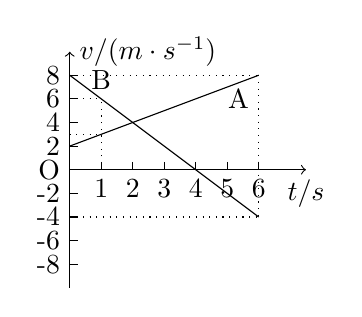
\begin{tikzpicture}
  \draw [->](0,0)--(3,0) node [anchor=north]{$t/s$};
  \draw [->](0,-1.5)--(0,1.5) node [anchor=west]{$v/(m\cdot s^{-1})$};
  \draw (0,0) node [anchor=east] {O};
  \draw (0.4,0.1)--(0.4,0) node [anchor=north] {1};
  \draw (0.8,0.1)--(0.8,0) node [anchor=north] {2};
  \draw (1.2,0.1)--(1.2,0) node [anchor=north] {3};
  \draw (1.6,0.1)--(1.6,0) node [anchor=north] {4};
  \draw (2.0,0.1)--(2.0,0) node [anchor=north] {5};
  \draw (2.4,0.1)--(2.4,0) node [anchor=north] {6};
  \draw (0.1,0.3)--(0,0.3) node [anchor=east]{2};
  \draw (0.1,0.6)--(0,0.6) node [anchor=east]{4};
  \draw (0.1,0.9)--(0,0.9) node [anchor=east]{6};
  \draw (0.1,1.2)--(0,1.2) node [anchor=east]{8};
  \draw (0.1,-0.3)--(0,-0.3) node [anchor=east]{-2};
  \draw (0.1,-0.6)--(0,-0.6) node [anchor=east]{-4};
  \draw (0.1,-0.9)--(0,-0.9) node [anchor=east]{-6};
  \draw (0.1,-1.2)--(0,-1.2) node [anchor=east]{-8};
  \draw (0,0.3) --(2.4,1.2);
  \draw (0,1.2) --(2.4,-0.6);
  \draw [dotted] (0,1.2)--(2.4,1.2);
  \draw [dotted] (0,-0.6)--(2.4,-0.6);
  \draw [dotted] (2.4,1.2)--(2.4,-0.6);
  \draw [dotted] (0.4,0)--(0.4,0.9);
  \draw[dotted] (0,0.9)--(0.4,0.9);
  \draw[dotted] (0,0.45)--(0.4,0.45);
  \draw (0.4,0.9) node [anchor=south]{B};
  \draw (2.4,0.9) node [anchor=east]{A};
\end{tikzpicture}
:>
[1]A,B各做什么运动并求其加速度;
[2]两图象交点的意义;
[3]求$1s$ A,B的速度;
[4]求$6s$ 末A,B的速度.
  
a.见解析

e.(1) A物体沿规定的正方向做匀加速直线运动,加速度大小为 $a_1=\frac{v-v_0}{t}=\frac{8-2}{6}m/s^2=1m/s^2$ ,方向与初速度方向相同;B物体前$4s$沿规定的正方向做匀减速直线运动,$4s$ 后沿反方向做匀加速直线运动,加速度为$a_2=\frac{0-8}{4}m/s^2=-2m/s^2$ ,负号表示加速度方向与初速度方向相反.
\newline
(2)两图象的交点表示在该时刻A,B速度相同.
\newline
(3)$1s$末A物体的速度为$3m/s$,和初速度方向相同;B物体的速度为$6m/s$ ,和初速度方向相同.
\newline
(4)$6s$ 末A物体的速度为$8m/s$ ,和初速度方向相同;B物体的速度为$-4m/s$,和初速度方向相反.

2.一物体从静止开始以$2m/s^2$ 的加速度做匀加速直线运动,经过$5s$ 后做匀速直线运动,最后$2s$ 的时间内物体做匀减速直线运动直到静止.求
[1]物体做匀加速直线运动时速度大小;
[2]物体做匀减速直线运动时的加速度.

a.(1) $10m/s$ (2) $-5m/s^2$ ,加速度方向与$v_c$ 方向相反.

e.此题先画出草图如
<:
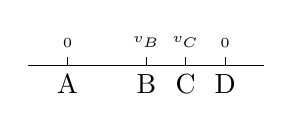
\begin{tikzpicture}
 \draw (0,0)--(3,0);
 \draw (0.5,0)node[anchor=north]{A}--(0.5,0.1) node [anchor=south] {\tiny $0$};
 \draw (1.5,0)node[anchor=north]{B}--(1.5,0.1) node [anchor=south] {\tiny $v_B$};
 \draw (2,0)node[anchor=north]{C}--(2,0.1) node [anchor=south] {\tiny $v_C$};
 \draw (2.5,0)node[anchor=north]{D}--(2.5,0.1) node [anchor=south] {\tiny $0$};
\end{tikzpicture}
:>
所示,设图中$A\rightarrow B$ 为匀加速直线运动,$B \rightarrow C$为匀速直线运动,$C\rightarrow D$为匀减速直线运动,$BC$段的速度为$AB$段的末速度,也是$CD$ 段的初速度.
\newline
(1)由速度与时间的关系\eqref{eq:v-t}式得
$$v_B=a_1t_1=2\times 5 m/s=10m/s$$
即做匀速直线运动的速度为$10m/s$
\newline
(2)由加速度的定义\eqref{eq:acceleration}式得
$$a_2=\cfrac{v-v_0}{t_2}=\cfrac{v_D-v_C}{t_2}=\cfrac{0-10}{2}m/s^2=-5m/s^2$$
负号表示加速度方向与$v_C$方向相反.

\end{calculate}
